\documentclass{beamer}[10]
\usepackage{pgf}
\usepackage[english]{babel}
\usepackage[utf8]{inputenc}
\usepackage{beamerthemesplit}
\usepackage{graphics,epsfig, subfigure}
\usepackage{url}
\usepackage{srcltx}
\usepackage{hyperref}

\definecolor{kugreen}{RGB}{50,61,93}
\definecolor{kugreenlys}{RGB}{132,139,158}
\definecolor{kugreenlyslys}{RGB}{173,177,190}
\definecolor{kugreenlyslyslys}{RGB}{214,216,223}
\setbeamercovered{transparent}
\mode<presentation>
\usetheme[numbers,totalnumber,compress,sidebarshades]{PaloAlto}
\setbeamertemplate{footline}[frame number]

\usecolortheme[named=kugreen]{structure}
\useinnertheme{circles}
\usefonttheme[onlymath]{serif}
\setbeamercovered{transparent}
\setbeamertemplate{blocks}[rounded][shadow=true]

% \logo{\includegraphics[width=0.8cm]{KULogo}}
%\useoutertheme{infolines}
\title{Predict email open}
\author{Manuel Felipe Pineda}
\institute{Introduction to data science \\
Universidad Tecnologica de Pereira}
\date{\today}


\begin{document}
\frame{\titlepage \vspace{-0.5cm}
}

\frame
{
  \frametitle{Overview}
  \tableofcontents%[pausesection]
}

\section{Experiments}

\frame{
  \frametitle{Experiments}
  Each experiment was tested using the cross-validation technique
  with the k-fold method, with k equals to 10, in order to evaluate the
  estimators performance. \cite{scikit-learn} \cite{sklearn-api}

  Each experiment was evaluated based in the f1-score and the
  accuracy-score, were run in 4 cores  and 4 GB of RAM
  \footnote{Intel(R) Core(TM) i5-4300U CPU}
}

\frame{
  \frametitle{Dimensionality reduction}
  \begin{columns}
\column{0.5\textwidth}
  \begin{figure}
    \centering
    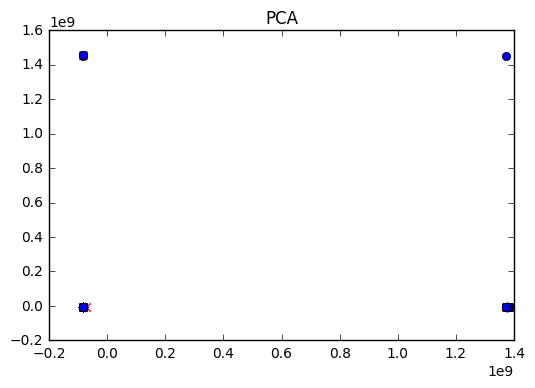
\includegraphics[width=0.9\textwidth]{../img/pca.png}
    \caption{\label{fig:pca} PCA}
  \end{figure}
\column{0.5\textwidth}
  \begin{figure}
    \centering
    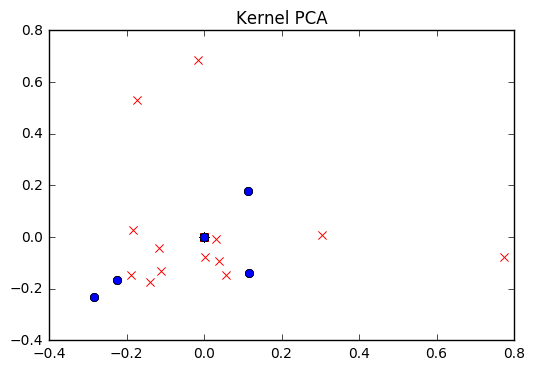
\includegraphics[width=0.9\textwidth]{../img/kpca.png}
    \caption{\label{fig:kpca} Kernel - PCA}
  \end{figure}
\end{columns}
}

\section{Estimators}

\frame[allowframebreaks]{
  \frametitle{Estimators}
  \begin{table}[]
    \centering
    \caption{Comparison between estimators}
    \label{tab:estimators}
    \resizebox{\linewidth}{!}{
      \begin{tabular}{llll}
        \hline
        \multicolumn{1}{l}{\textbf{Method}} & \multicolumn{1}{l}{\textbf{Accuracy}} & \multicolumn{1}{l}{\textbf{F1 Score}} & \multicolumn{1}{l}{\textbf{Time (s)}} \\ \hline
        \textbf{Linear models} & & & \\ \hline
        Perceptron & 0.60 (+/- 0.35) & 0.37 (+/- 0.21) & 15.18  \\
        Logistic Regression & 0.72 (+/- 0.00) & 0.28 (+/- 0.01) & 68.48 \\
        Stochastic GD & 0.68 (+/- 0.23) & 0.30 (+/- 0.25) & 15.49 \\
        SGD log reg as loss & 0.60 (+/- 0.35) & 0.39 (+/- 0.22) & 15.78 \\
        Passive Aggressive Classifier & 0.56 (+/- 0.38) & 0.37 (+/- 0.21) & 23.27 \\
        \textbf{Non linear transformation} & & & \\ \hline
        SVC & 0.67 (+/- 0.01) & 0.02 (+/- 0.02) & 28.05 \\
        NuSVC & 0.67 (+/- 0.00) & 0.01 (+/- 0.02) & 29.39 \\
        Random Trees Embbedings & 0.72 (+/- 0.00) & 0.28 (+/- 0.01) & 141.27 \\
        Extra Trees Classifier \footnote{This classifier is able to
        get perfect score using the whole data set}
        & 0.70 (+/- 0.03) & 0.41 (+/- 0.06) & 1.25 \\

    \end{tabular}}
  \end{table}

  \newpage

  \frametitle{Estimators}
  \begin{table}[]
    \centering
    \caption{Comparison between estimators}
    \label{tab:estimators2}
    \resizebox{\linewidth}{!}{
      \begin{tabular}{llll}
        \hline
        \multicolumn{1}{l}{\textbf{Method}} & \multicolumn{1}{l}{\textbf{Accuracy}} & \multicolumn{1}{l}{\textbf{F1 Score}} & \multicolumn{1}{l}{\textbf{Time (s)}} \\ \hline
        Naive Bayes & 0.68 (+/- 0.00) & 0.41 (+/- 0.01) & 41.89 \\
        RBF Sampler (Kernel approx) & 0.64 (+/- 0.03) & 0.16 (+/- 0.08)
        & 1.54 \\
        \textbf{Manifold Learning} & & & \\ \hline
        K Neighbors Classifier & 0.61 (+/- 0.04) & 0.41 (+/- 0.05) & 1.58 \\
        Radius Neighbors Classifier & 0.67 (+/- 0.00) & 0.00 (+/- 0.00) & 12.97 \\
        \textbf{ANN} & & & \\ \hline
        Multilayer Perceptron & 0.33 (+/- 0.00) & 0.50 (+/- 0.00) & 11.18 \\
    \end{tabular}}
  \end{table}
}

\section{Tuning hyperparameters}

\frame{
  \frametitle{Tuning hyperparameters}
  The method Exhaustive Grid Search was used to optimize
  the hyperparameters of the best estimators (f1-score)
  \begin{itemize}
    \item Multilayer Perceptron: 0.5
    \item K Neighbors: 0.41
    \item Extra Trees Classifier: 0.51
  \end{itemize}
}

\section{Conclusions}

\frame[allowframebreaks]{
  \frametitle{Conclusions}

  \vspace{0.5cm}

  The current data is very complex, as result, most of the
  classifiers get bad performance, even worse that random. However,
  it is possible to configure some estimators in order to receive
  better score that pure chance.

  \vspace{0.5cm}

  This process is very demanding in terms of time and processing
  because needs to explore a wide range of hyperparameters and the
  execution becomes exponential in the number of hyperparameters.

  \newpage

  By the way, if we compare the score with respect the official
  leaderboard for the contest, this solution would result in the
  place 80 of 500.
}
\section{References}

\frame[allowframebreaks]{
  \frametitle{References}
  {\scriptsize
    \bibliography{mybib}{}
  }
  \bibliographystyle{unsrt}
}

\end{document}
